\documentclass{csse4400}

%\teachermodetrue

\usepackage{tikz}
\usetikzlibrary{positioning}
\usetikzlibrary{arrows}

\usepackage{float}

\usepackage{enumitem}

\usepackage{languages}

\title{SpamOverflow}
\author{Evan Hughes \& Richard Thomas}

\date{\week[tutorial]{11}}
\begin{document}

\maketitle


\section{Brief}

Design a service for scanning and filtering spam/malicious emails.
Specially the service needs to support:
\begin{itemize}
    \item Scanning an email via an API request.
    \item Providing access to a specified REST API, e.g. for use by front-end interfaces and internal teams.
    \item Remaining responsive while scanning emails.
\end{itemize}

\paragraph{Task}
You are working for SpamOverflow,
a new competitor in the email security space.
Spam\-Overflow uses a microservices based architecture to implement their new malicious email filtering platform.
The CEO saw on your resume that you are taking Software Architecture and has assigned you to design and implement a service.
This service must be scalable to cope with a large influx of emails.

\paragraph{Requirements}
Email filtering software can filter email as it arrives or after.
SpamOverflow will implement a service that does not impede the flow of traffic (i.e. does not prevent email from arriving).
It will receive an API call when the mail server receives an email message.
The service then pulls the email from the user's inbox, as fast as it can,
to prevent the user from seeing the malicious email or clicking any links.

Commercial email providers send an API request for each email received.
For optimal performance this service needs to be able to handle a large number of requests in a short period of time.

Since these emails can be dangerous, the service must be able to report that it is bad or good in a timely manner.
Though genuine emails that are incorrectly marked as dangerous should be returned to the user as quickly as possible.

Persistence is an important characteristic of the platform.
Customers will want to analyse why emails were flagged after the fact.
Upon receiving an email scan request, and after filtering,
the system must guarantee that the data has been saved to persistent storage before returning a success response.


\section{Outline}

\subsection*{Introduction (5 minutes)}
Introduction to the brief and resources,
including the \link{API specification}{https://csse6400.uqcloud.net/api/spamoverflow}
and quality scenarios in section \ref{sec:scenarios}.
Your service will use a tool to scan emails for malicious content,
called \link{SpamHammer}{https://github.com/CSSE6400/SpamHammer}.

\subsection*{Planning (10 minutes)}
In small groups, discuss the following issues or any others you think are relevant to designing the service.

\begin{enumerate}
    \item What are the key requirements introduced by the quality scenarios?
    \item What strategies can you implement to support these scenarios?
    \item What AWS resources would prove helpful?
    \item What are the likely bottlenecks?
\end{enumerate}

%TODO Teacher notes need to be replaced to be relevant to SpamOverflow.
\teacher{
    \subsection{What are the key requirements introduced by the quality scenarios?}

    \begin{itemize}
        \item Q1, Q2, Q3 all introduce load to the system for ticket purchasing.
        \item Q4 introduces load on the concerts endpoint for every purchase.
        \item Q5 introduces the need to handle load on the same endpoint for multiple entries
                 and the printing of tickets at scale.
        \item Q6 adds priorities to the mix for ticket printing.
        \item Q7 adds the need to cancel / alter async process that are in flight.
        \item Q8 introduces a large amount of load that ids expected to push the system to the limit.
              Designers should expect that it could crash and need to recover.
        \item API specifies that concert seating must be updated within 3 minutes.
    \end{itemize}
}
\teacher{
    \subsection{What strategies can you implement to support these scenarios?}

    \paragraph{Ticket Rendering}
    Looking at the \link{hamilton documentation}{https://github.com/CSSE6400/hamilton},
    we have been given the expected runtime and memory usage to create an individual ticket.
    We can see that the process is CPU intensive but light on memory, taking a few seconds to generate a ticket.
    We could possibly get away with running this process sequentially,
    but with the CPU resources required we may want to offload processing.

    \textcolor{purple}{\textbf{+ Queue Ticket Rendering to offload processing.}}
}
\teacher{
    \paragraph{Ticket Priority}
    From the scenarios, we can see that there is a significant amount of time between the two concerts,
    so we could apply more novel approaches to the problem.

    \begin{itemize}
        \item Create buckets of priority and assign jobs based on the concert time compared to today's date.
              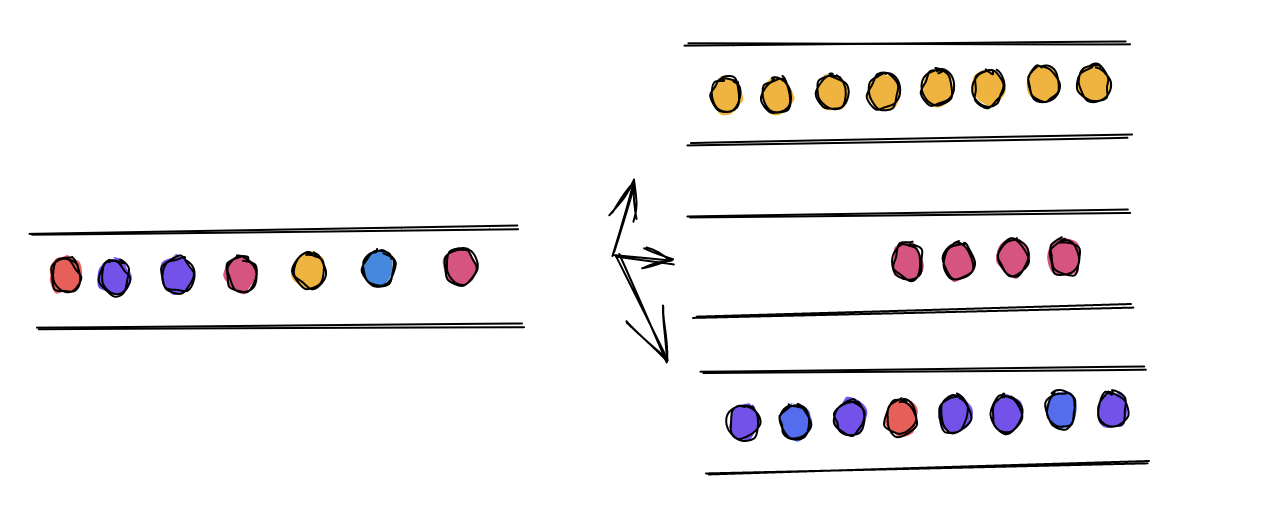
\includegraphics[width=0.73\textwidth]{images/bucket-queue.png}
        \item Stage queued jobs into a table,
              where a queue manager selectively pulls jobs from the table based on priority.
              \textcolor{red}{The queue manager would keep the queue fed with a small amount of jobs
              such that it is just enough for the workers.}
              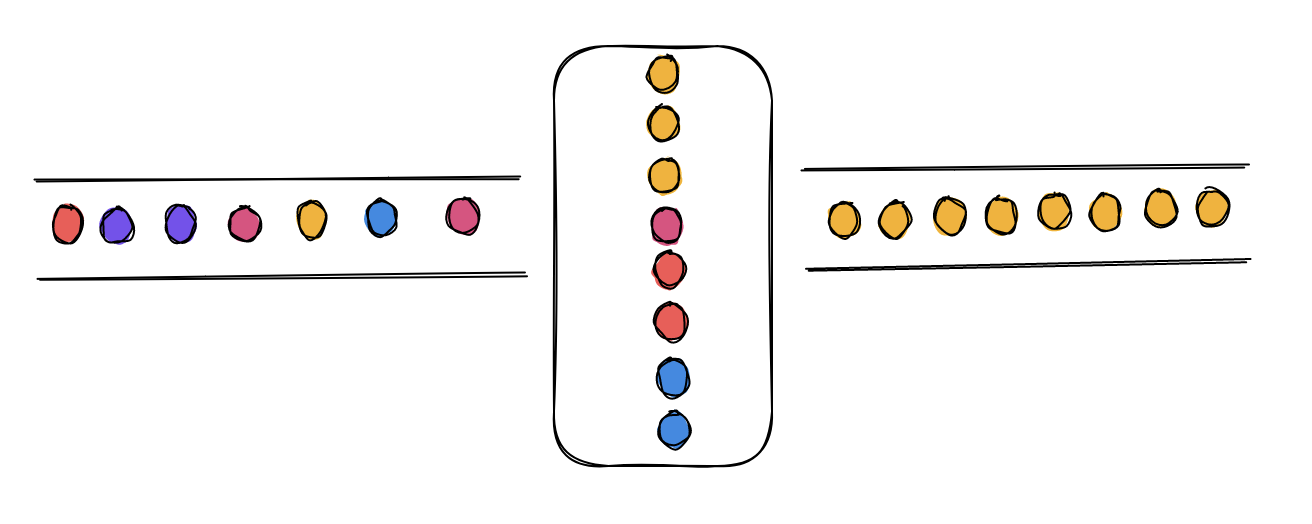
\includegraphics[width=0.73\textwidth]{images/staging-queue.png}
    \end{itemize}

    \textcolor{purple}{\textbf{+ Buckets for priority due to simplicity but the staging table is more versatile}}
}
\teacher{
    \paragraph{Seating Rendering}
    As above we see that seating requires more time due to CPU load but is relatively the same.
    We must proactively render the seating to ensure that we can meet the 3 minute requirement.
    Some strategies for this include:

    \begin{itemize}
        \item Render with every ticket purchase.
              \textcolor{red}{Means we cannot render tickets in parallel if they also render the seating.}
        \item Queue a render for every purchase.
        \item Queue on an exclusive queue for every purchase.
              \textcolor{red}{A queue that only allows one of every ID to be in the queue at a time.}
        \item Cron to render seating every minute if there are more tickets than the last render.
    \end{itemize}

    The exclusive queue design would allow for seating to be updated as fast as possible,
    while also reducing the resources required in large loads.
    On the other hand, the cron job is an elegantly simple design, while also meeting the expectations of users.

    \textcolor{purple}{\textbf{+ Cron to queue rendering of seating.}}
}
\teacher{
    \paragraph{Printing Invalidation}

    Depending on your queue implementation, you may be able to cancel jobs that are \textit{in flight}.
    By resetting the ticket status when our render job gets processed, it can skip the printing step.
    To avoid race conditions we can use a lock on the concert when changes are being processed.

    Another option would be storing a concert version identifier in each ticket,
    and when printing a ticket getting the current version identifier of the concert.
    When requesting a printed ticket we can check the versions,
    and if they do not match then we can invalidate the ticket.

    \textcolor{purple}{\textbf{+ Check ticket status during printing.}}
}
\teacher{
    \paragraph{Ticket Purchasing}
    Purchasing a ticket requires making sure that we have not oversold the concert.

    \begin{itemize}
        \item Count all tickets before selling a new one.
              \textcolor{red}{This can potentially allow overselling if two requests are made at the same time.}
        \item Lock the concert when selling a ticket.
              \textcolor{red}{This would cause a bottleneck on the concert endpoint.}
        \item Use an atomic counter to count the tickets sold for each concert.
        \item Use multiple atomic counters to distribute waiting for a lock.
              \textcolor{red}{By splitting the counters into buckets of tickets,
                              we can allow the client to randomly select a bucket,
                              which may have tickets available.}
    \end{itemize}

    \textcolor{purple}{\textbf{+ Use one or more atomic counters to count tickets.}}
}

\teacher{
    \subsection{What AWS resources would prove helpful?}

    \begin{itemize}
        \item Lambda for compute
        \item ECS for compute
        \item EC2 for compute
        \item DynamoDB for querying/caching/locking
        \item RDS for querying
        \item Redis for caching/locking/queueing
        \item S3 for storage
        \item SQS for queueing
    \end{itemize}
}

\teacher{
    \subsection{What are the likely bottlenecks?}

    Ticket purchasing is the most likely bottleneck, due to the use of atomic counters.
}

\subsection*{Design (20 minutes)}

In your group, design an appropriate architecture for SpamOverflow.
You need to consider the flow of an API request through your service,
use the \href{https://csse6400.uqcloud.net/api/spamoverflow}{API specification}
and quality scenarios in section \ref{sec:scenarios} to ensure all use cases have been considered.

\teacher{
    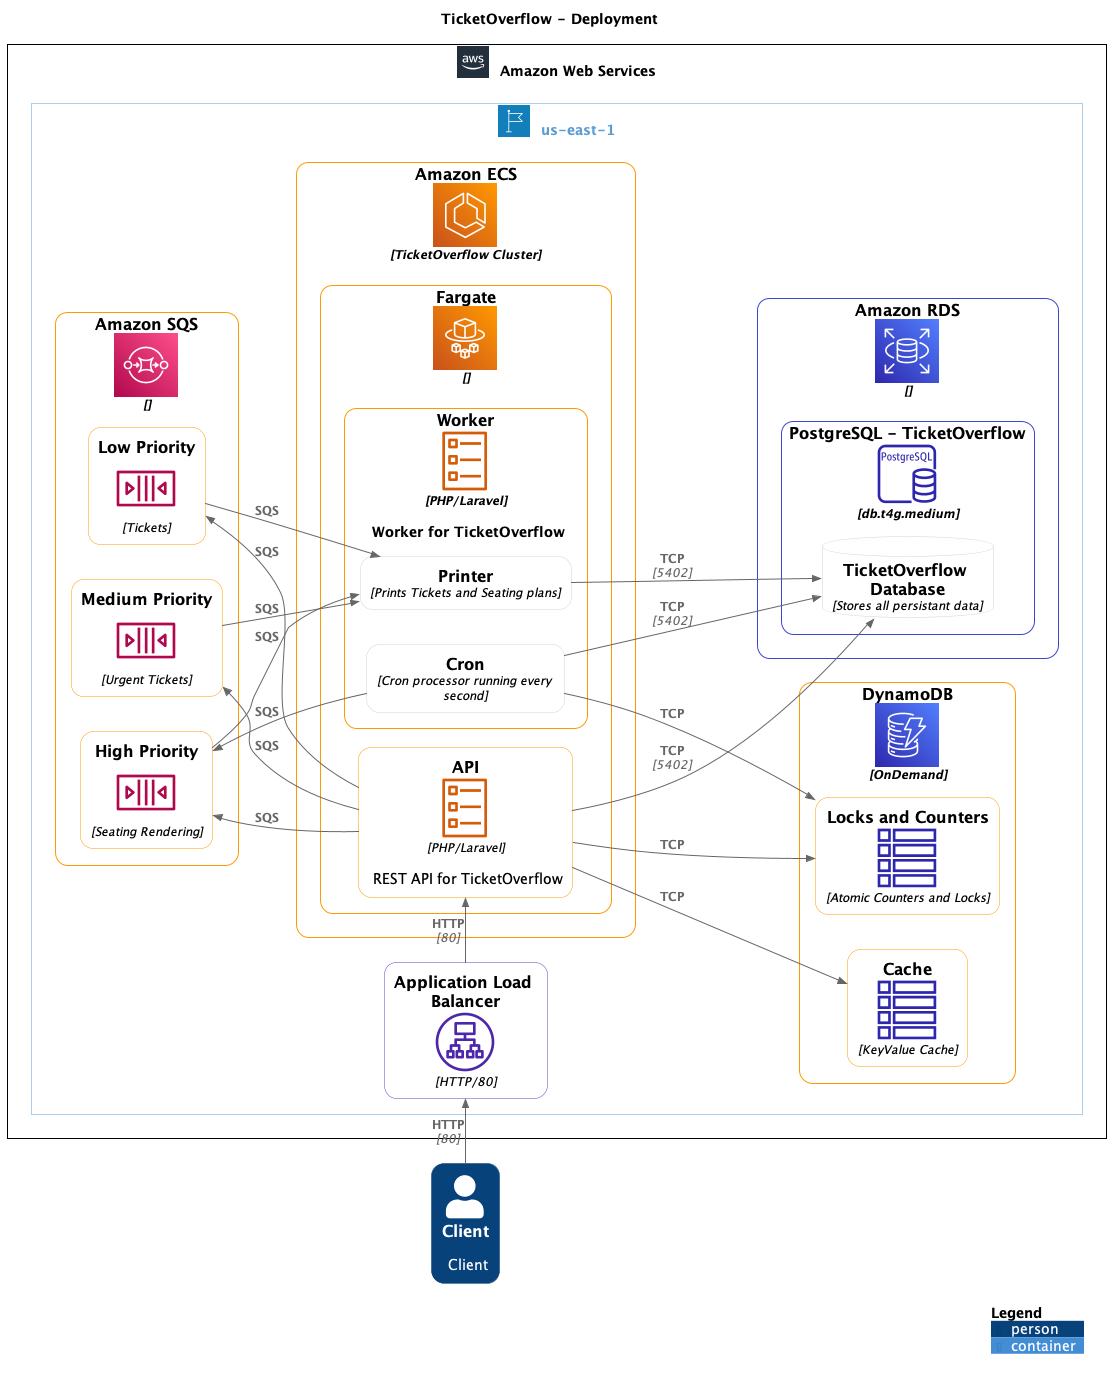
\includegraphics[width=\textwidth]{images/ticketoverflow.png}
}

\subsection*{Presentation (15 minutes)}

In the remaining time,
each group should present their proposed architecture design.
This is an opportunity for discussion amongst the class to point out limitations of the proposed system designs.


\section{Quality Scenarios}\label{sec:scenarios}

\paragraph{Q1: Steady Stream}
Steady receipt of email messages at a rate of \emph{M} per minute, fairly evenly spread across all customers.
Approximately 20\% of the messages are malicious.

\paragraph{Q2: Bad `News' Stream}
Steady receipt of email messages at a rate of \emph{N} per minute, fairly evenly spread across all customers.
Approximately 80\% of the messages are malicious.

\paragraph{Q3: Peaks and Troughs}
Periods of receipt of a high volume of email messages, followed by periods of low volume.

\paragraph{Q4: High Value Customer}
The Department of Defence (DoD) has adopted SpamOverflow.
They are a high value customer and you must ensure that their requests are handled quickly.
All other customers have a service level agreement (SLA) that guarantees a certain level of responsiveness.
You cannot ignore their requests to only prioritise the DoD's requests.

\paragraph{Q5: Leaked Directory}
A bad actor has managed to get the email addresses of all employees of <Large Company>.
They have sent a phishing email to all of the users advertising a pay raise with a link to a fake login page.
The email is sent to all 10,000 employees at the same time.

\paragraph{Q6: Personalised Attack}
A bad actor has trained an AI model using social media profiles of targeted victims.
They can generate personalised phishing email messages based on personal information.
As the messages are personalised, they can be of greatly different lengths and contain different content.
These messages can only be identified by SpamHammer.
They have sent these phishing messages to 2,000 users at the same time.

\end{document}
